\documentclass[a4paper, 12pt]{article}
\usepackage[left = 30mm, right = 30mm, top = 40mm, bottom = 30mm]{geometry}
%\usepackage[margin = 30cm]{geometry}
\usepackage{blindtext}
\usepackage{graphicx}
\usepackage{subcaption}
\usepackage{chemfig}
\usepackage{booktabs}
\usepackage{array}
\usepackage{document}
%\usepackage[table]{xcolor}

\usepackage{comment}
\usepackage{algorithm}
\usepackage{algorithmic}

\begin{document}
	\title{My first latex document}
	\author{author Name}
	\date{\today}
	\maketitle
	
	My First Latex Document
	
	\section{introduction}
	
	\subsection{Page setup}
	
	We have done our Latex document page setup
	
	\subsection {Title setup}
	
	\subsection{Writing text and paragraph}
	
	\blindtext \\
	\newline
	
	% \ double slash ka matlab two new line create hota hai
	
	\blindtext
	
	%\newpage
	\clearpage
	
	\section{Horizontal and Vertical spacing}
	\subsection{Horizontal Spacing}
	
	Horizontal \hspace{2in} spacing \\
	\\
	Horizontal \hfill spacing
	
	\subsection{Vertical spacing}
	vertical
	\vfill
	
	spacing
	\newpage
	\blindtext
	\vspace{5cm}
	\blindtext
	
	
	Now skip command in latex
	\blindtext
	
	\smallskip
	%\medskip
	%\bigskip
	
	\newpage
	
	\subsection{text formatting}
	\textbf{Boldface}. \\
	\textit{italics text}. \\
	
	\underline{underline text}. \\
	
	\noindent  Emphasizing text: \\ 
	We can now see the example of  
	\emph{emphasizing text}. \\
	\textit{We can now also
		\emph{emphasize}}.\\
	
	
	{\sffamily \blindtext}  % sansherif
	{\scshape \blindtext} % small cap
	\newpage
	\section{Inserting figure in latex}
	We have to use graphicx package.
	positioning of figure, we use htbp wgere h stand for here, b stand for bottom, t stand for top and p stand for new page.
	
	\begin{figure}
		\centering
		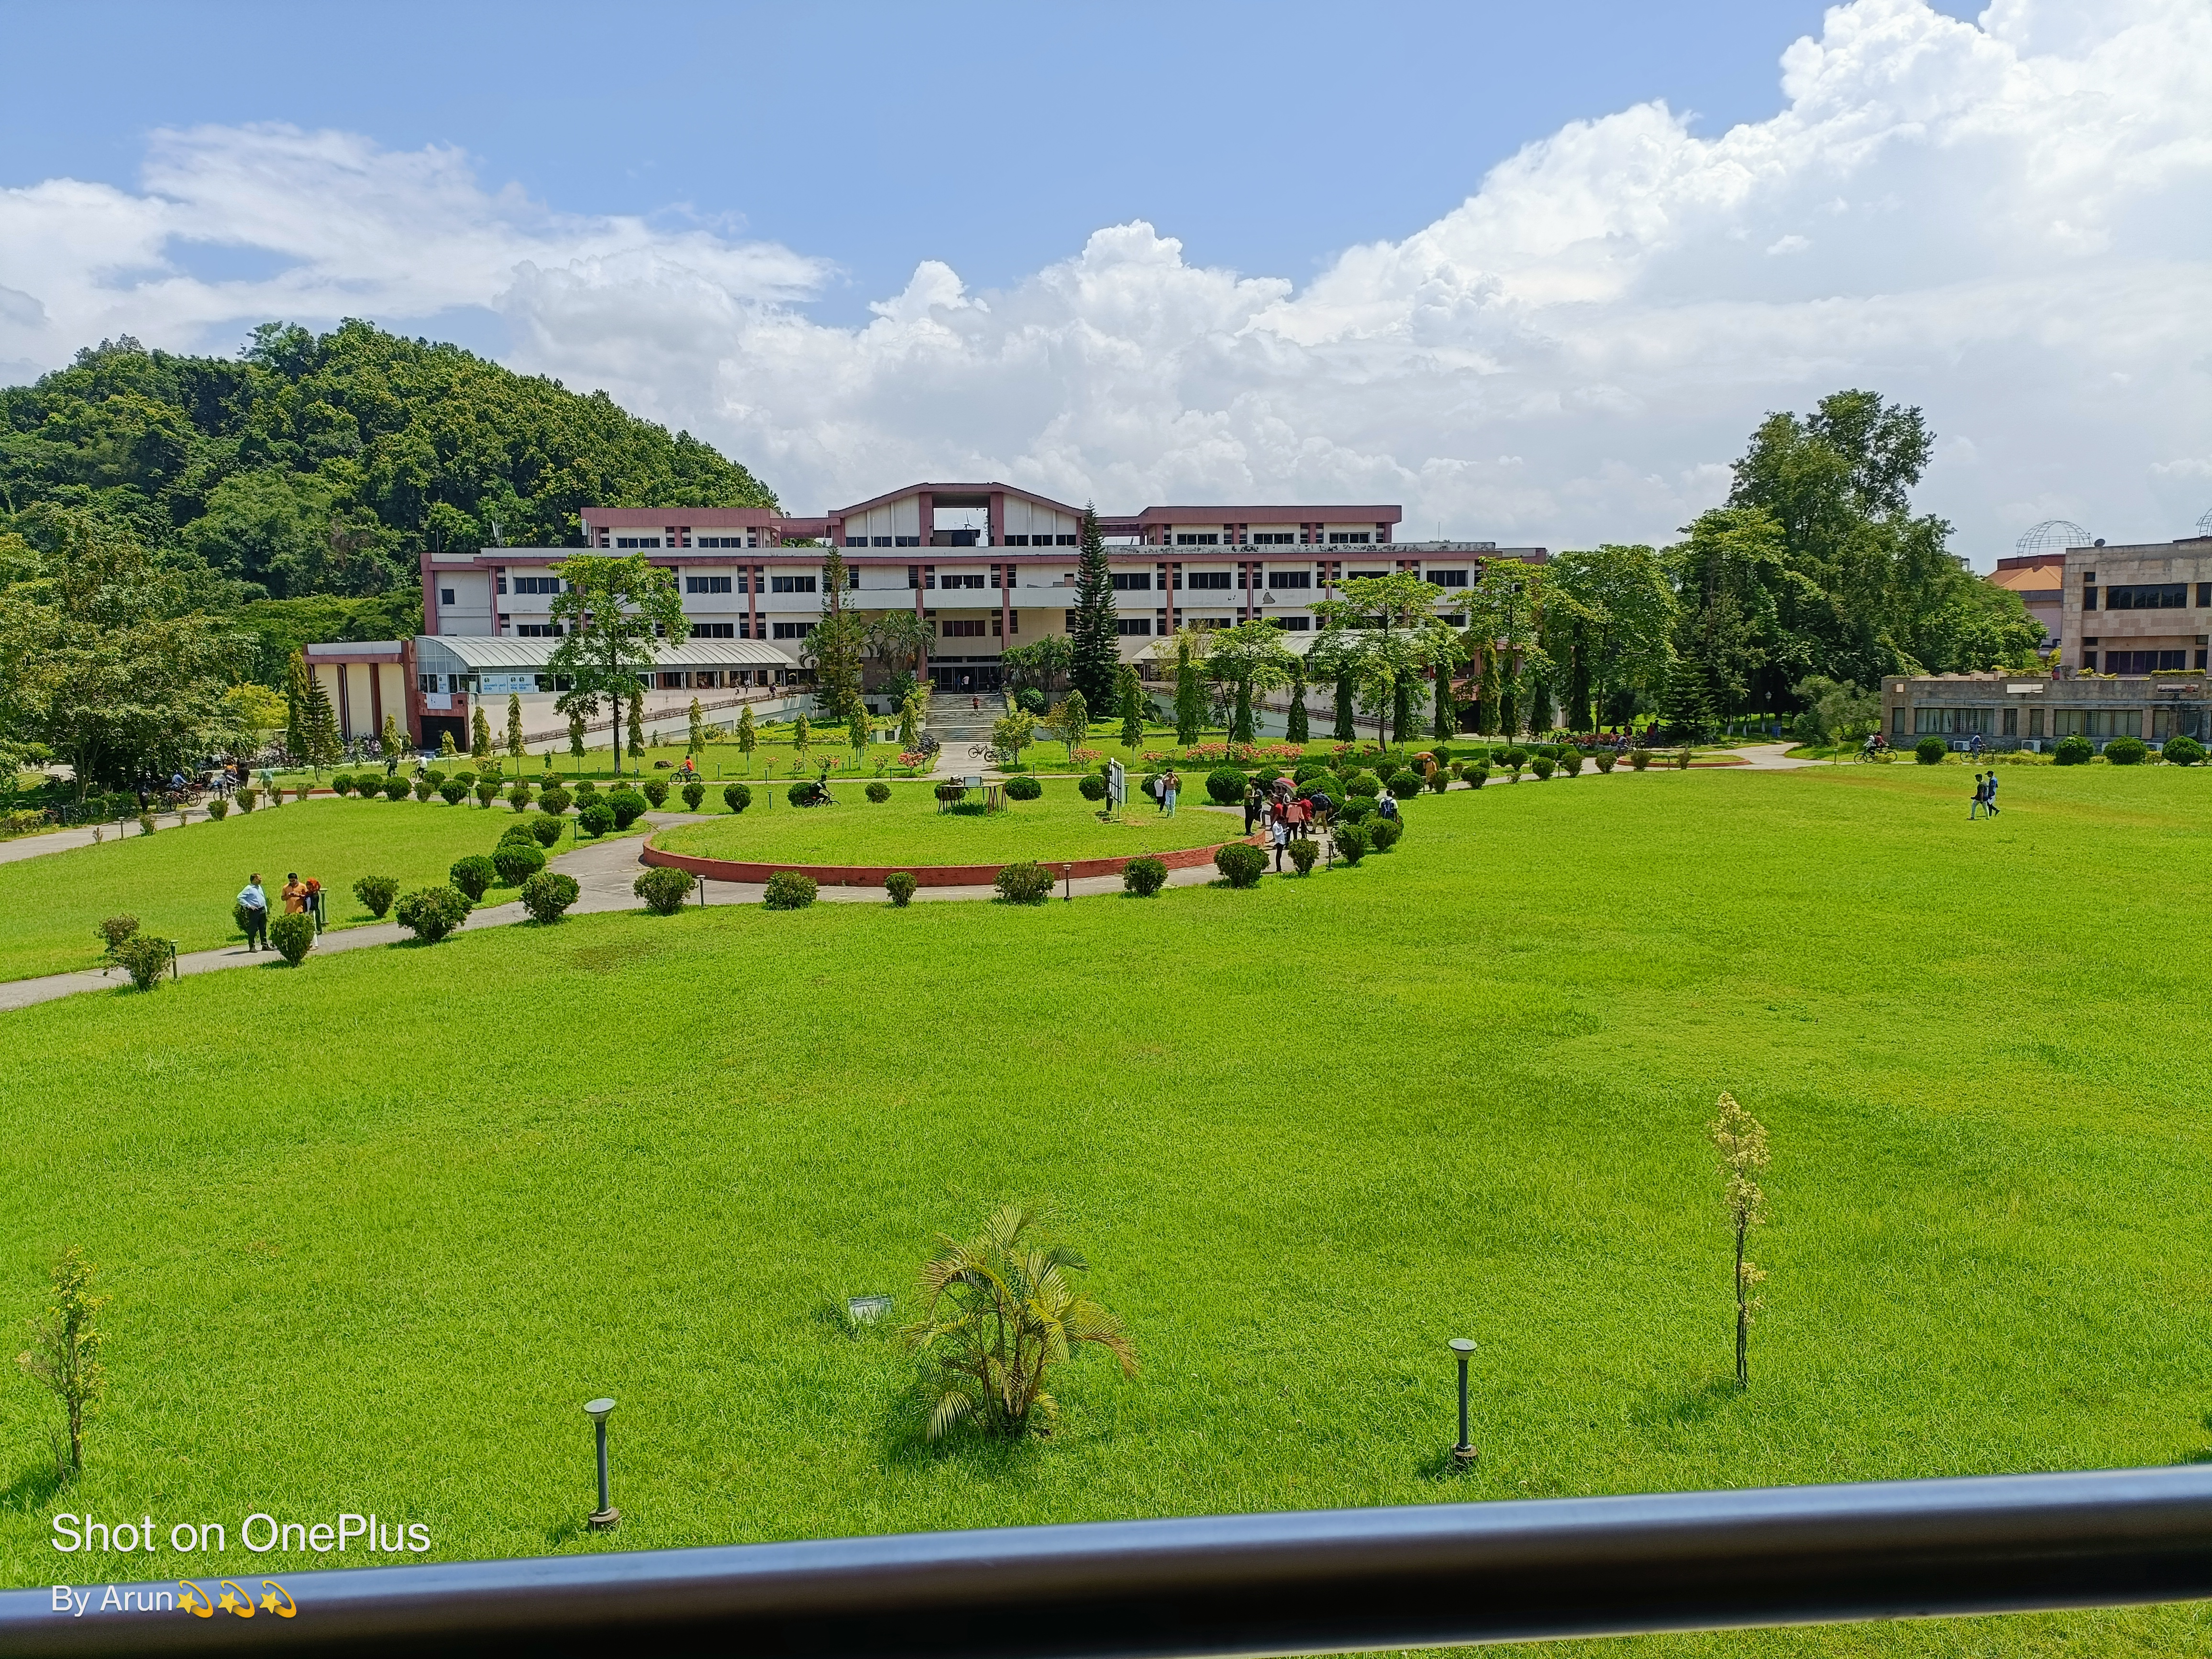
\includegraphics[scale=0.03, angle=45]{iitg.jpg}
		\caption{IITG LIBRARY}
	\end{figure}
	%\subsection{subfigure}
	\begin{figure}[h]
		\centering
		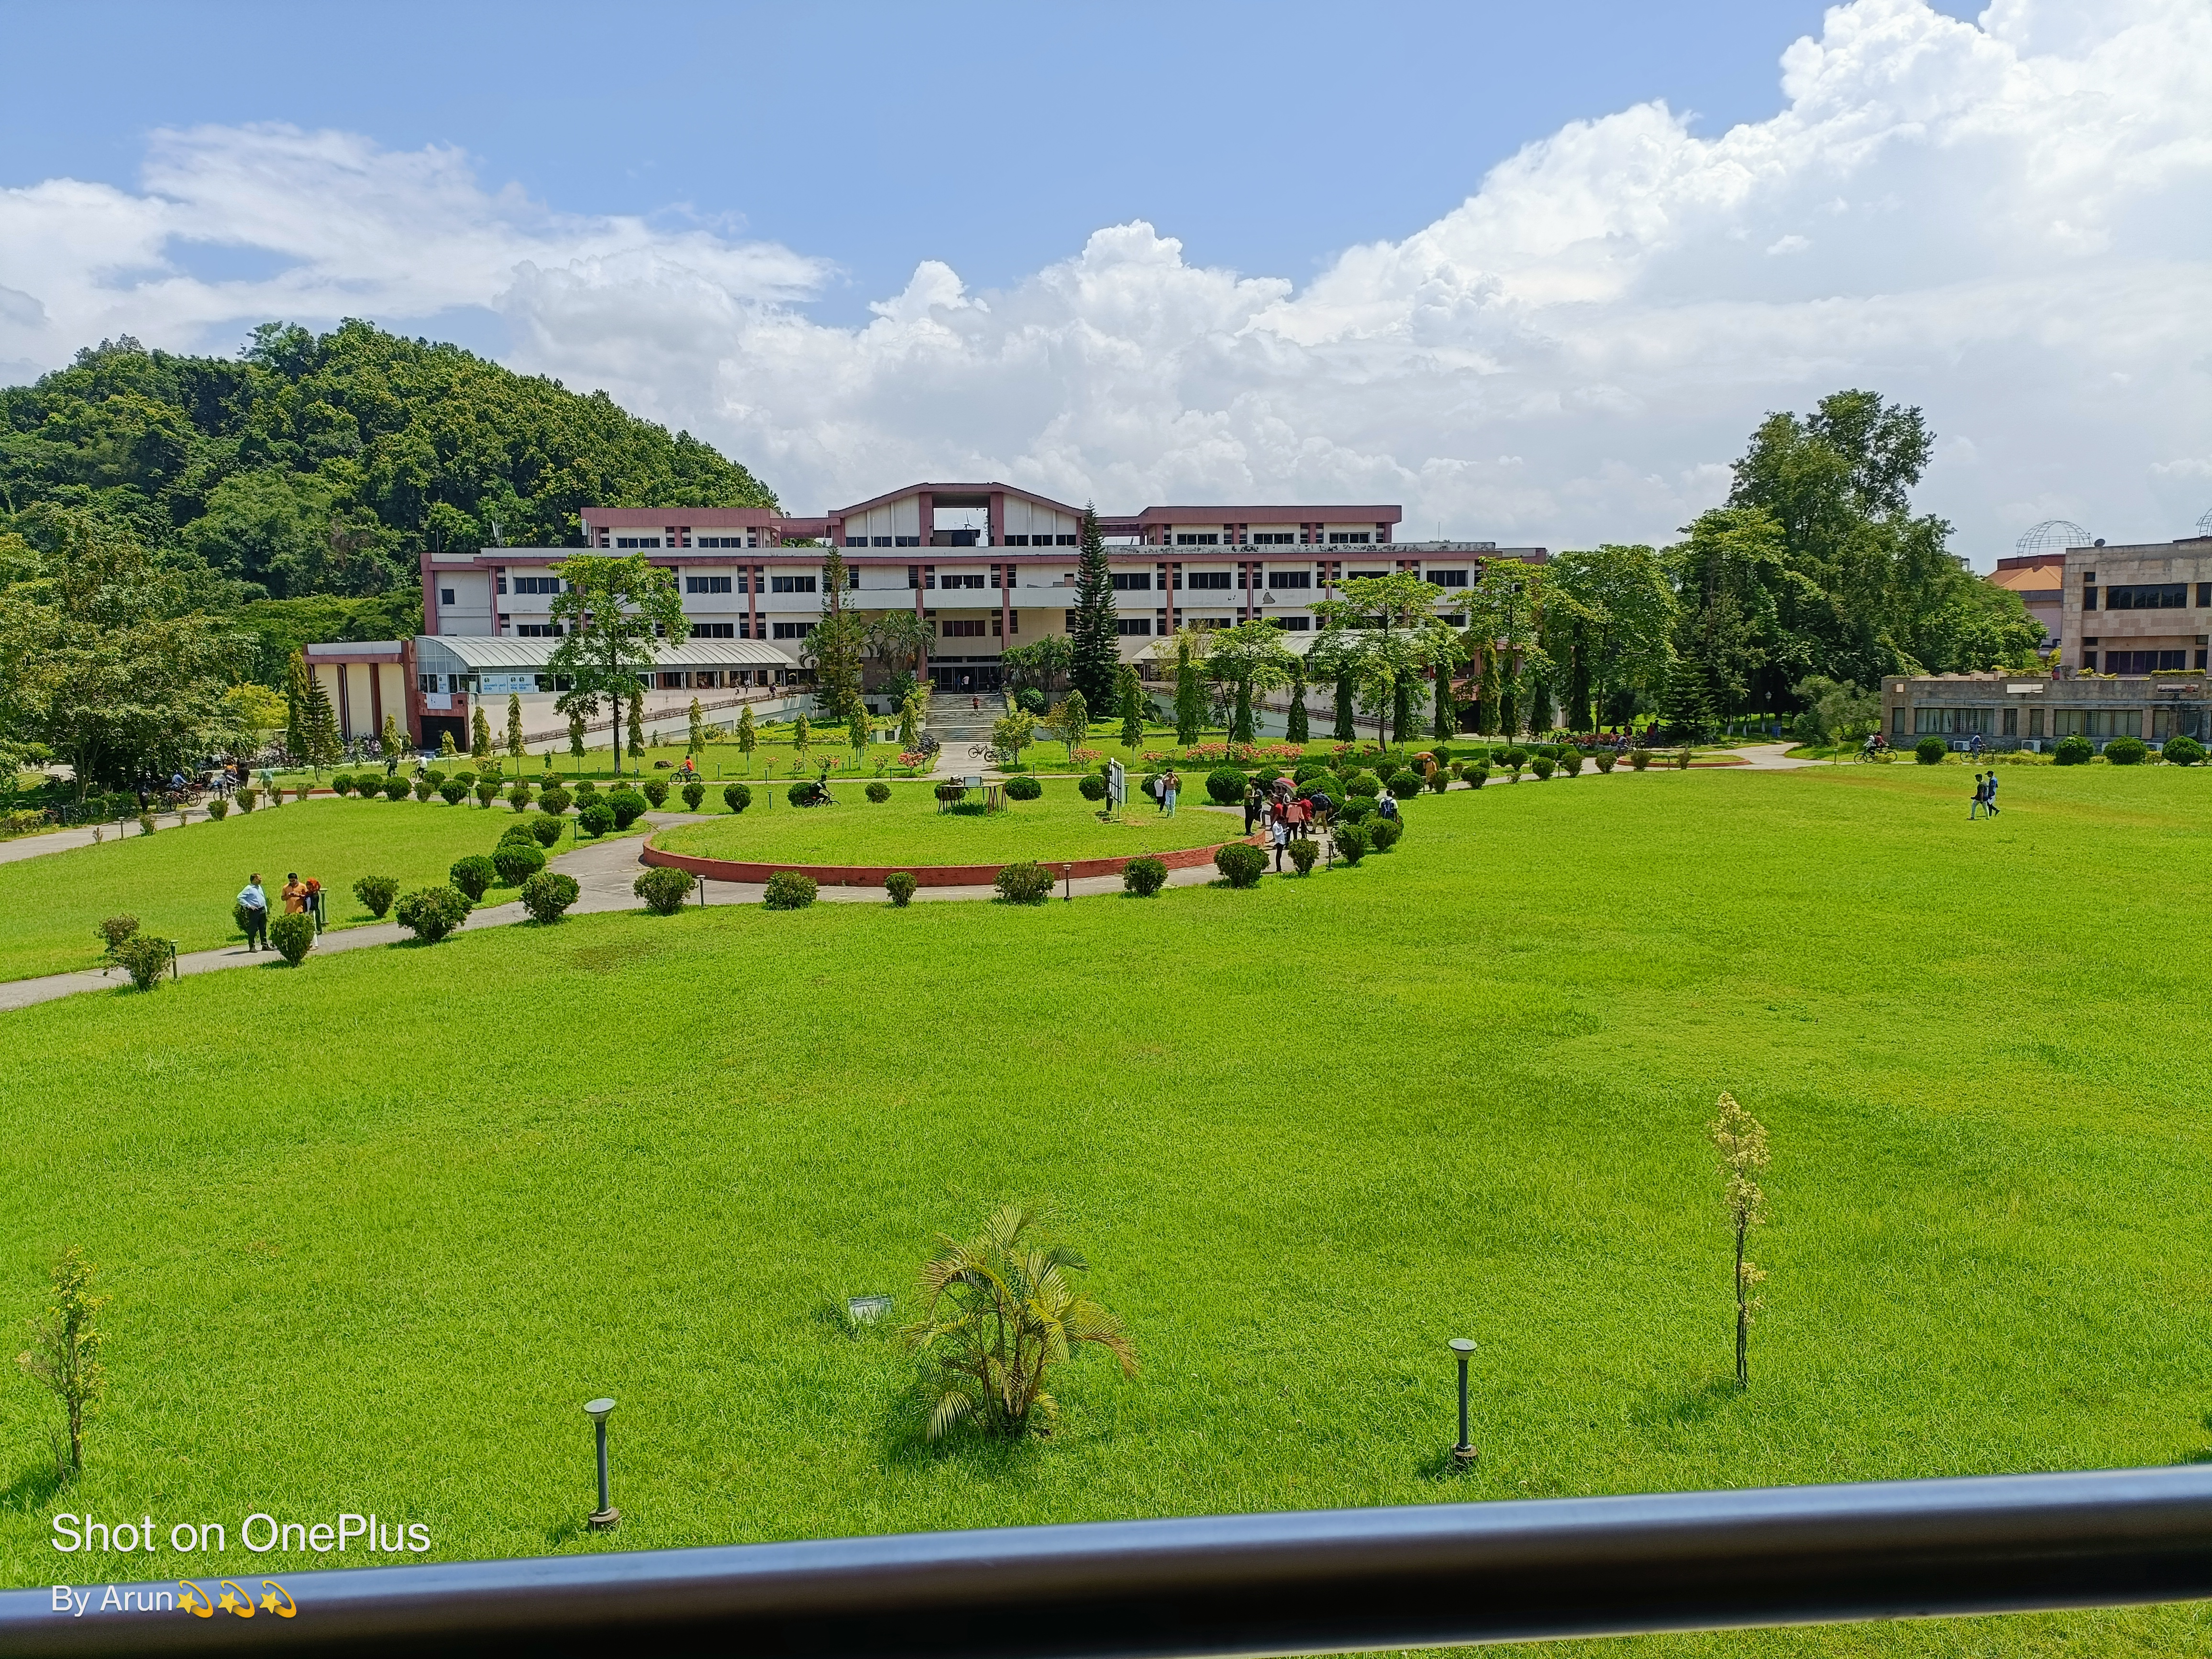
\includegraphics[width=10cm]{iitg.jpg}
		\caption{IITG LIBRARY}
		
	\end{figure}
	
	\subsection{subfigures}
	
	\begin{figure}[h]
		\begin{subfigure}{0.5\textwidth}
			\centering
			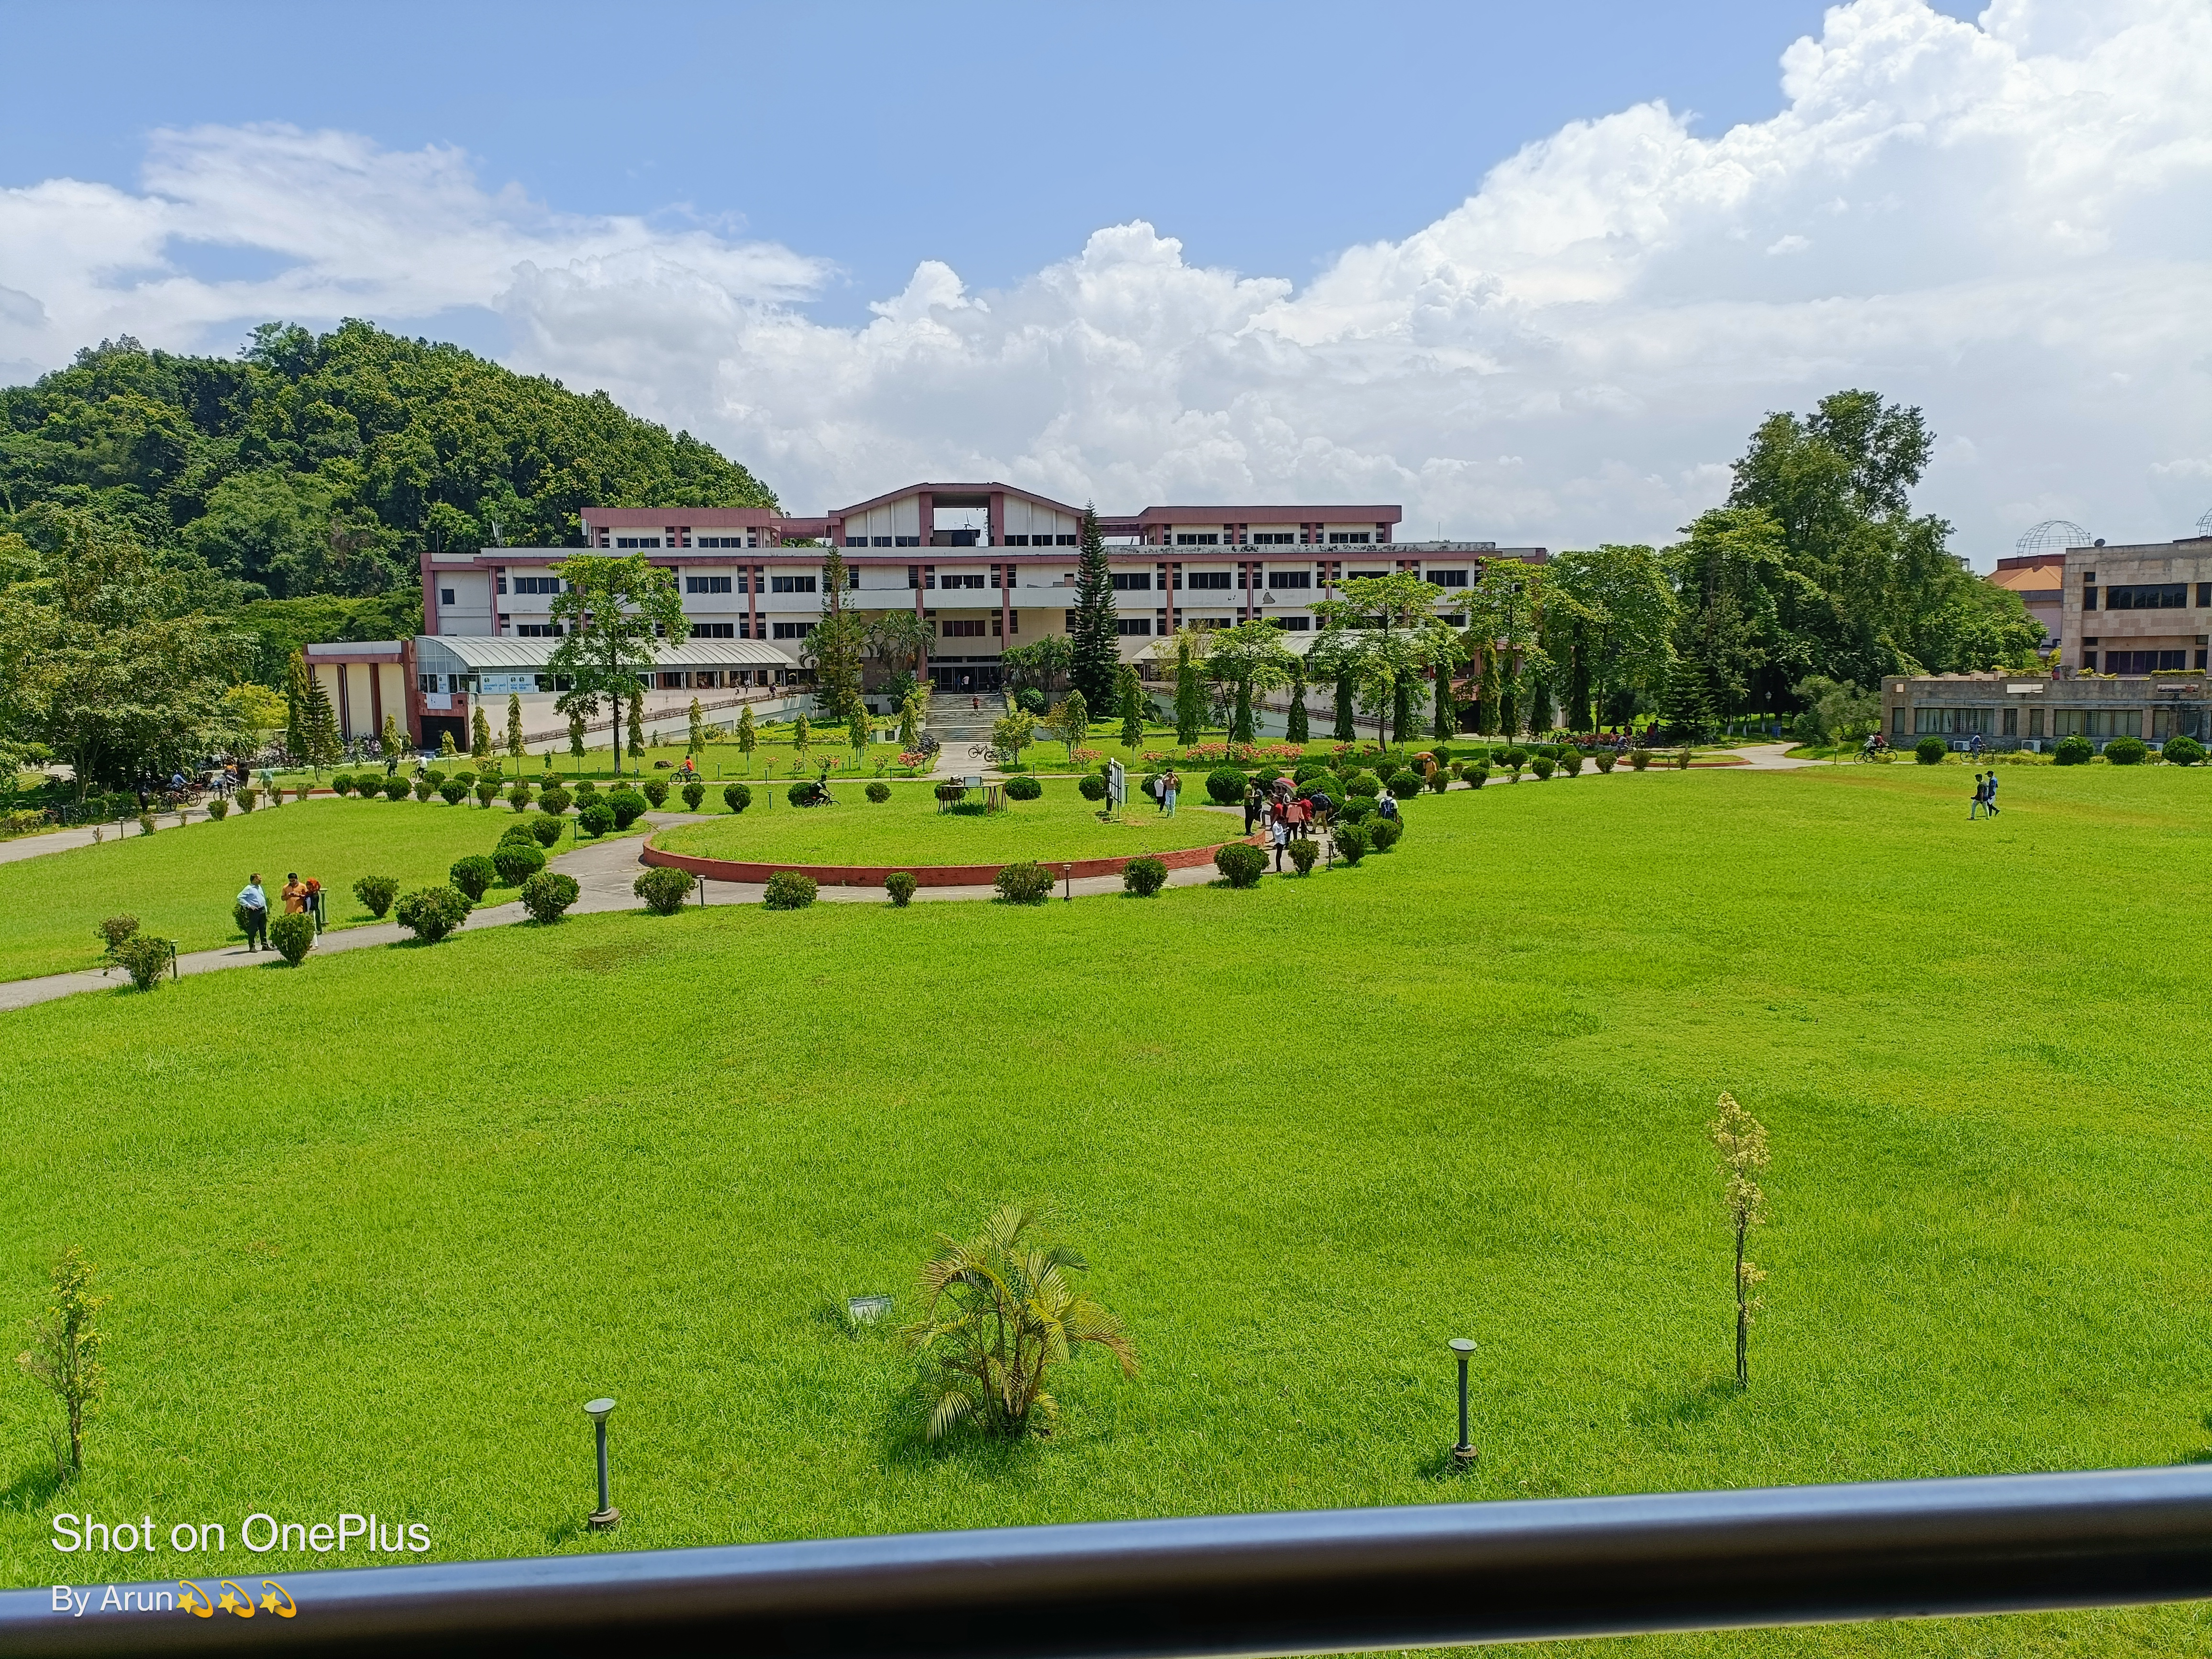
\includegraphics[scale=0.04]{iitg.jpg}
			\caption{IITG LIBRARY}
		\end{subfigure}
		\begin{subfigure}{0.5\textwidth}
			\centering
			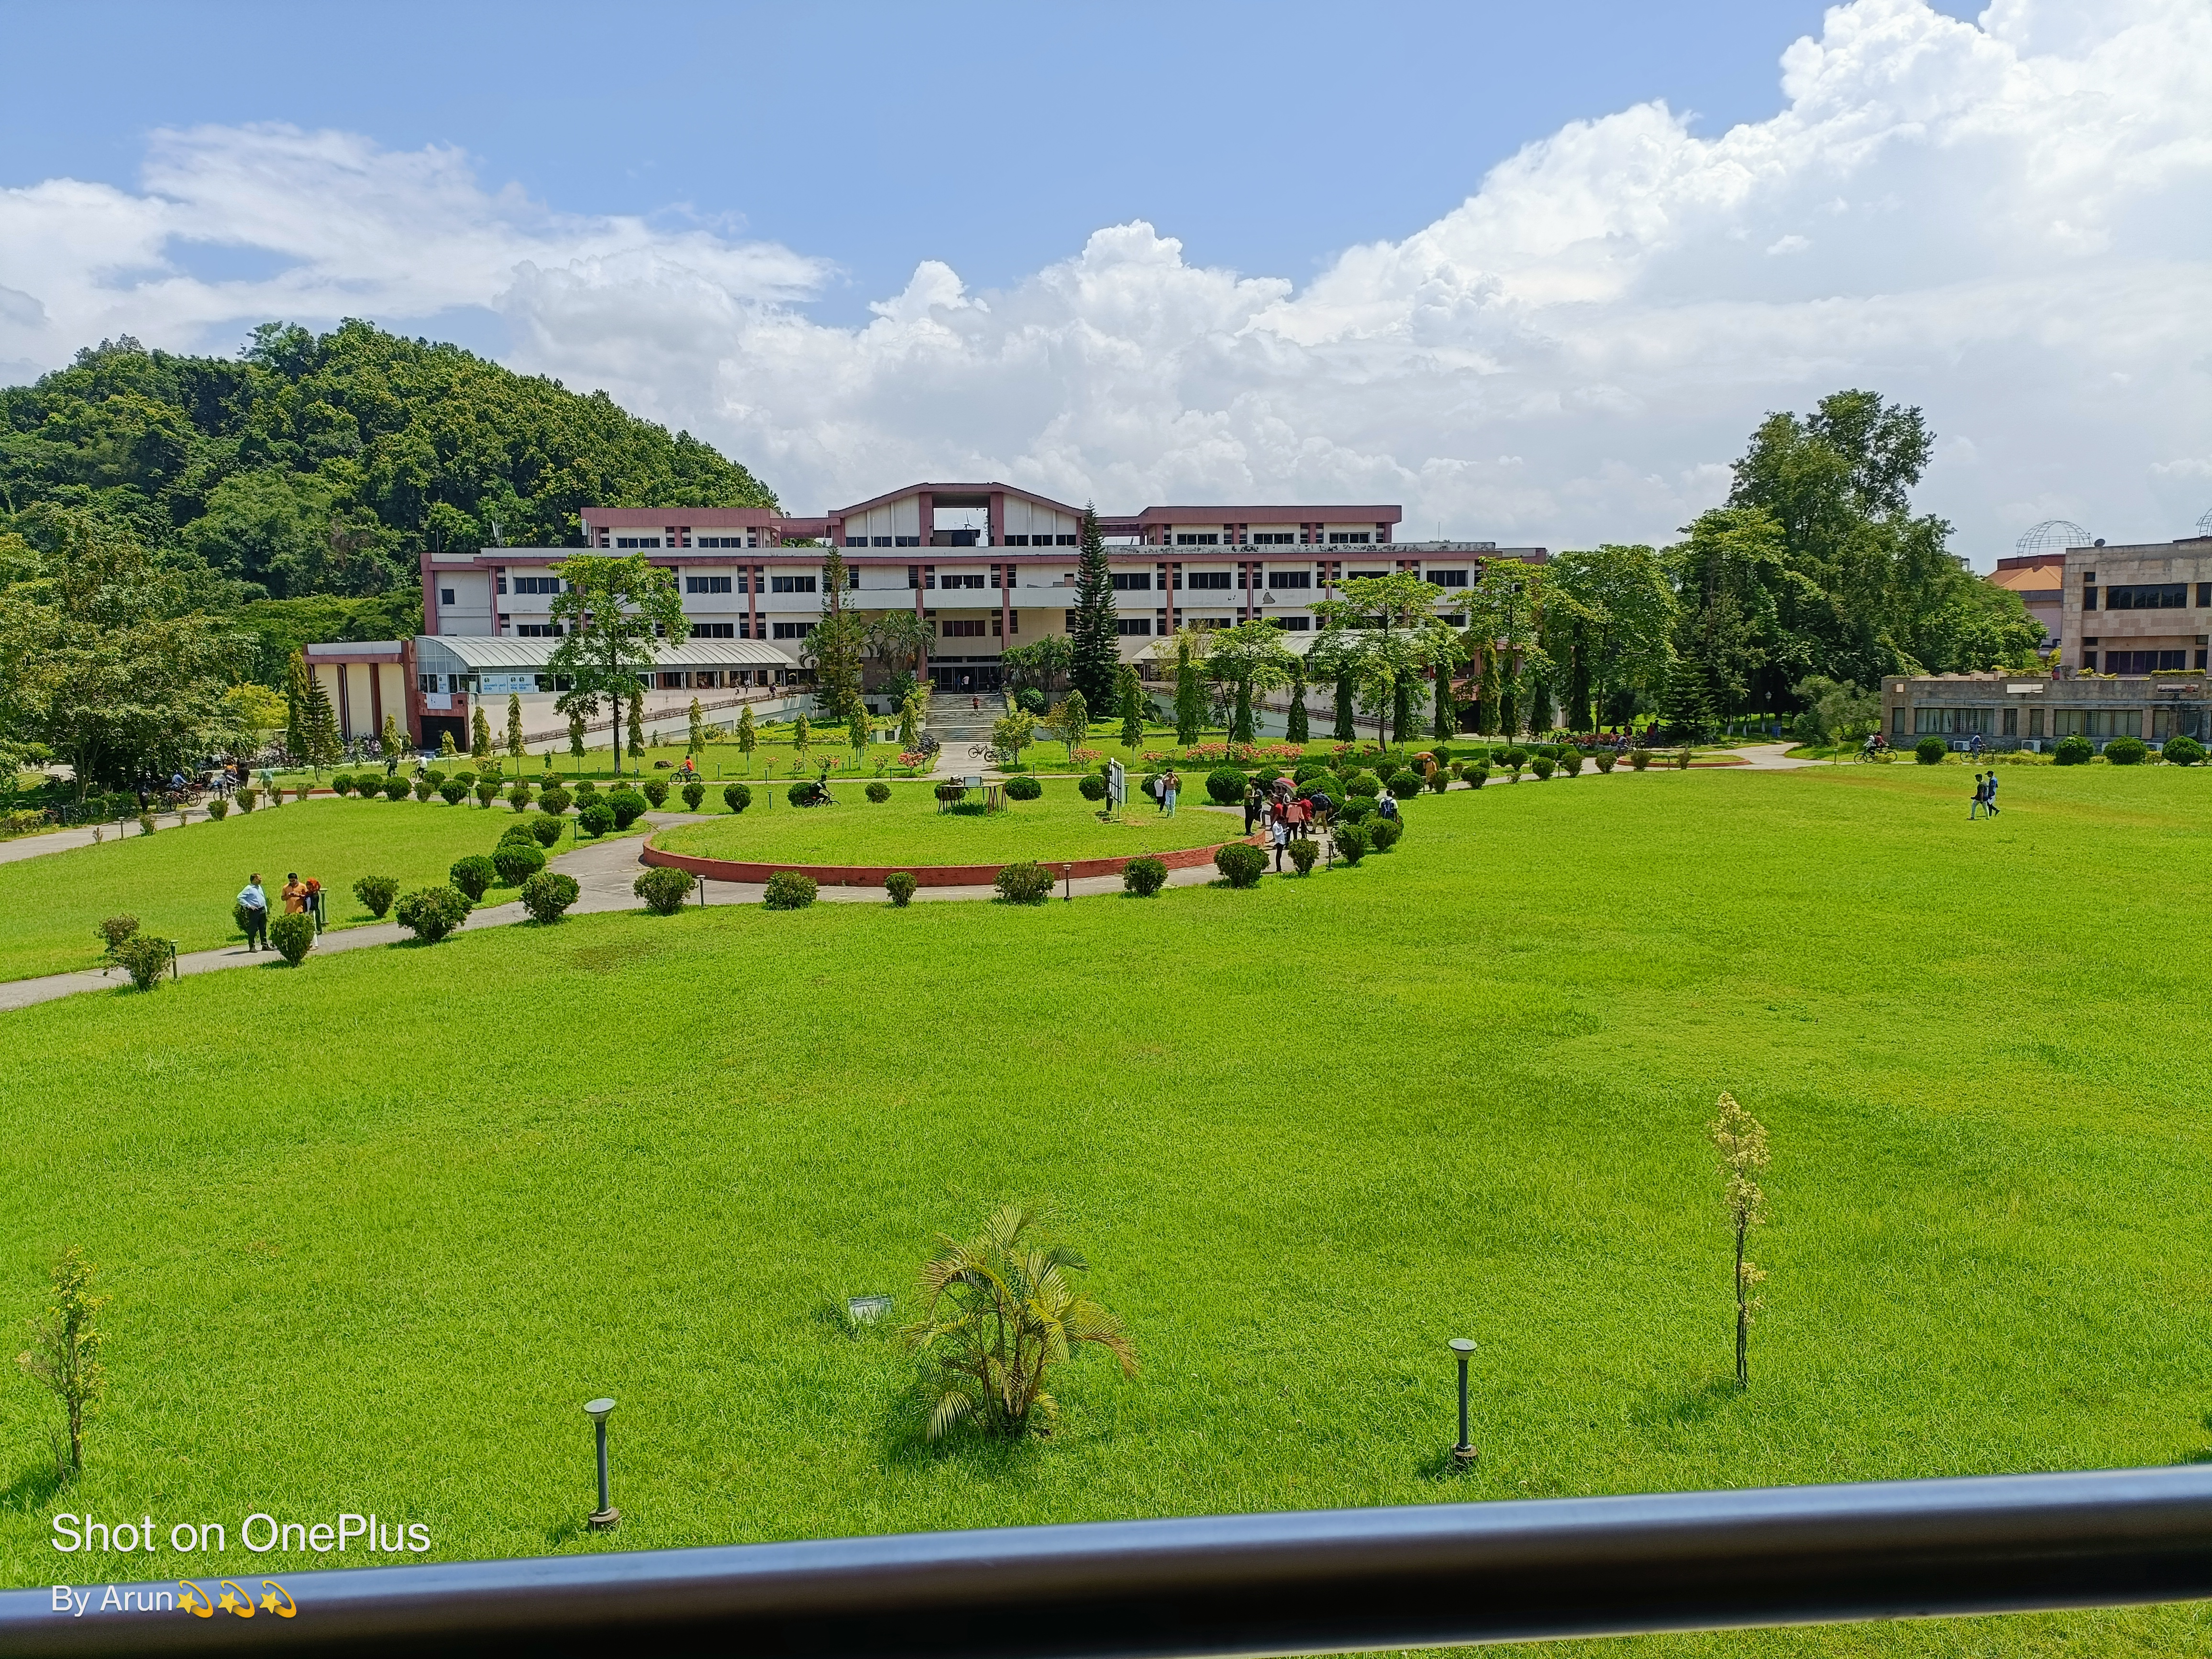
\includegraphics[scale=0.04]{iitg.jpg}
			\caption{IITG LIBRARY}
		\end{subfigure}
		\begin{subfigure}{0.5\textwidth}
			\centering
			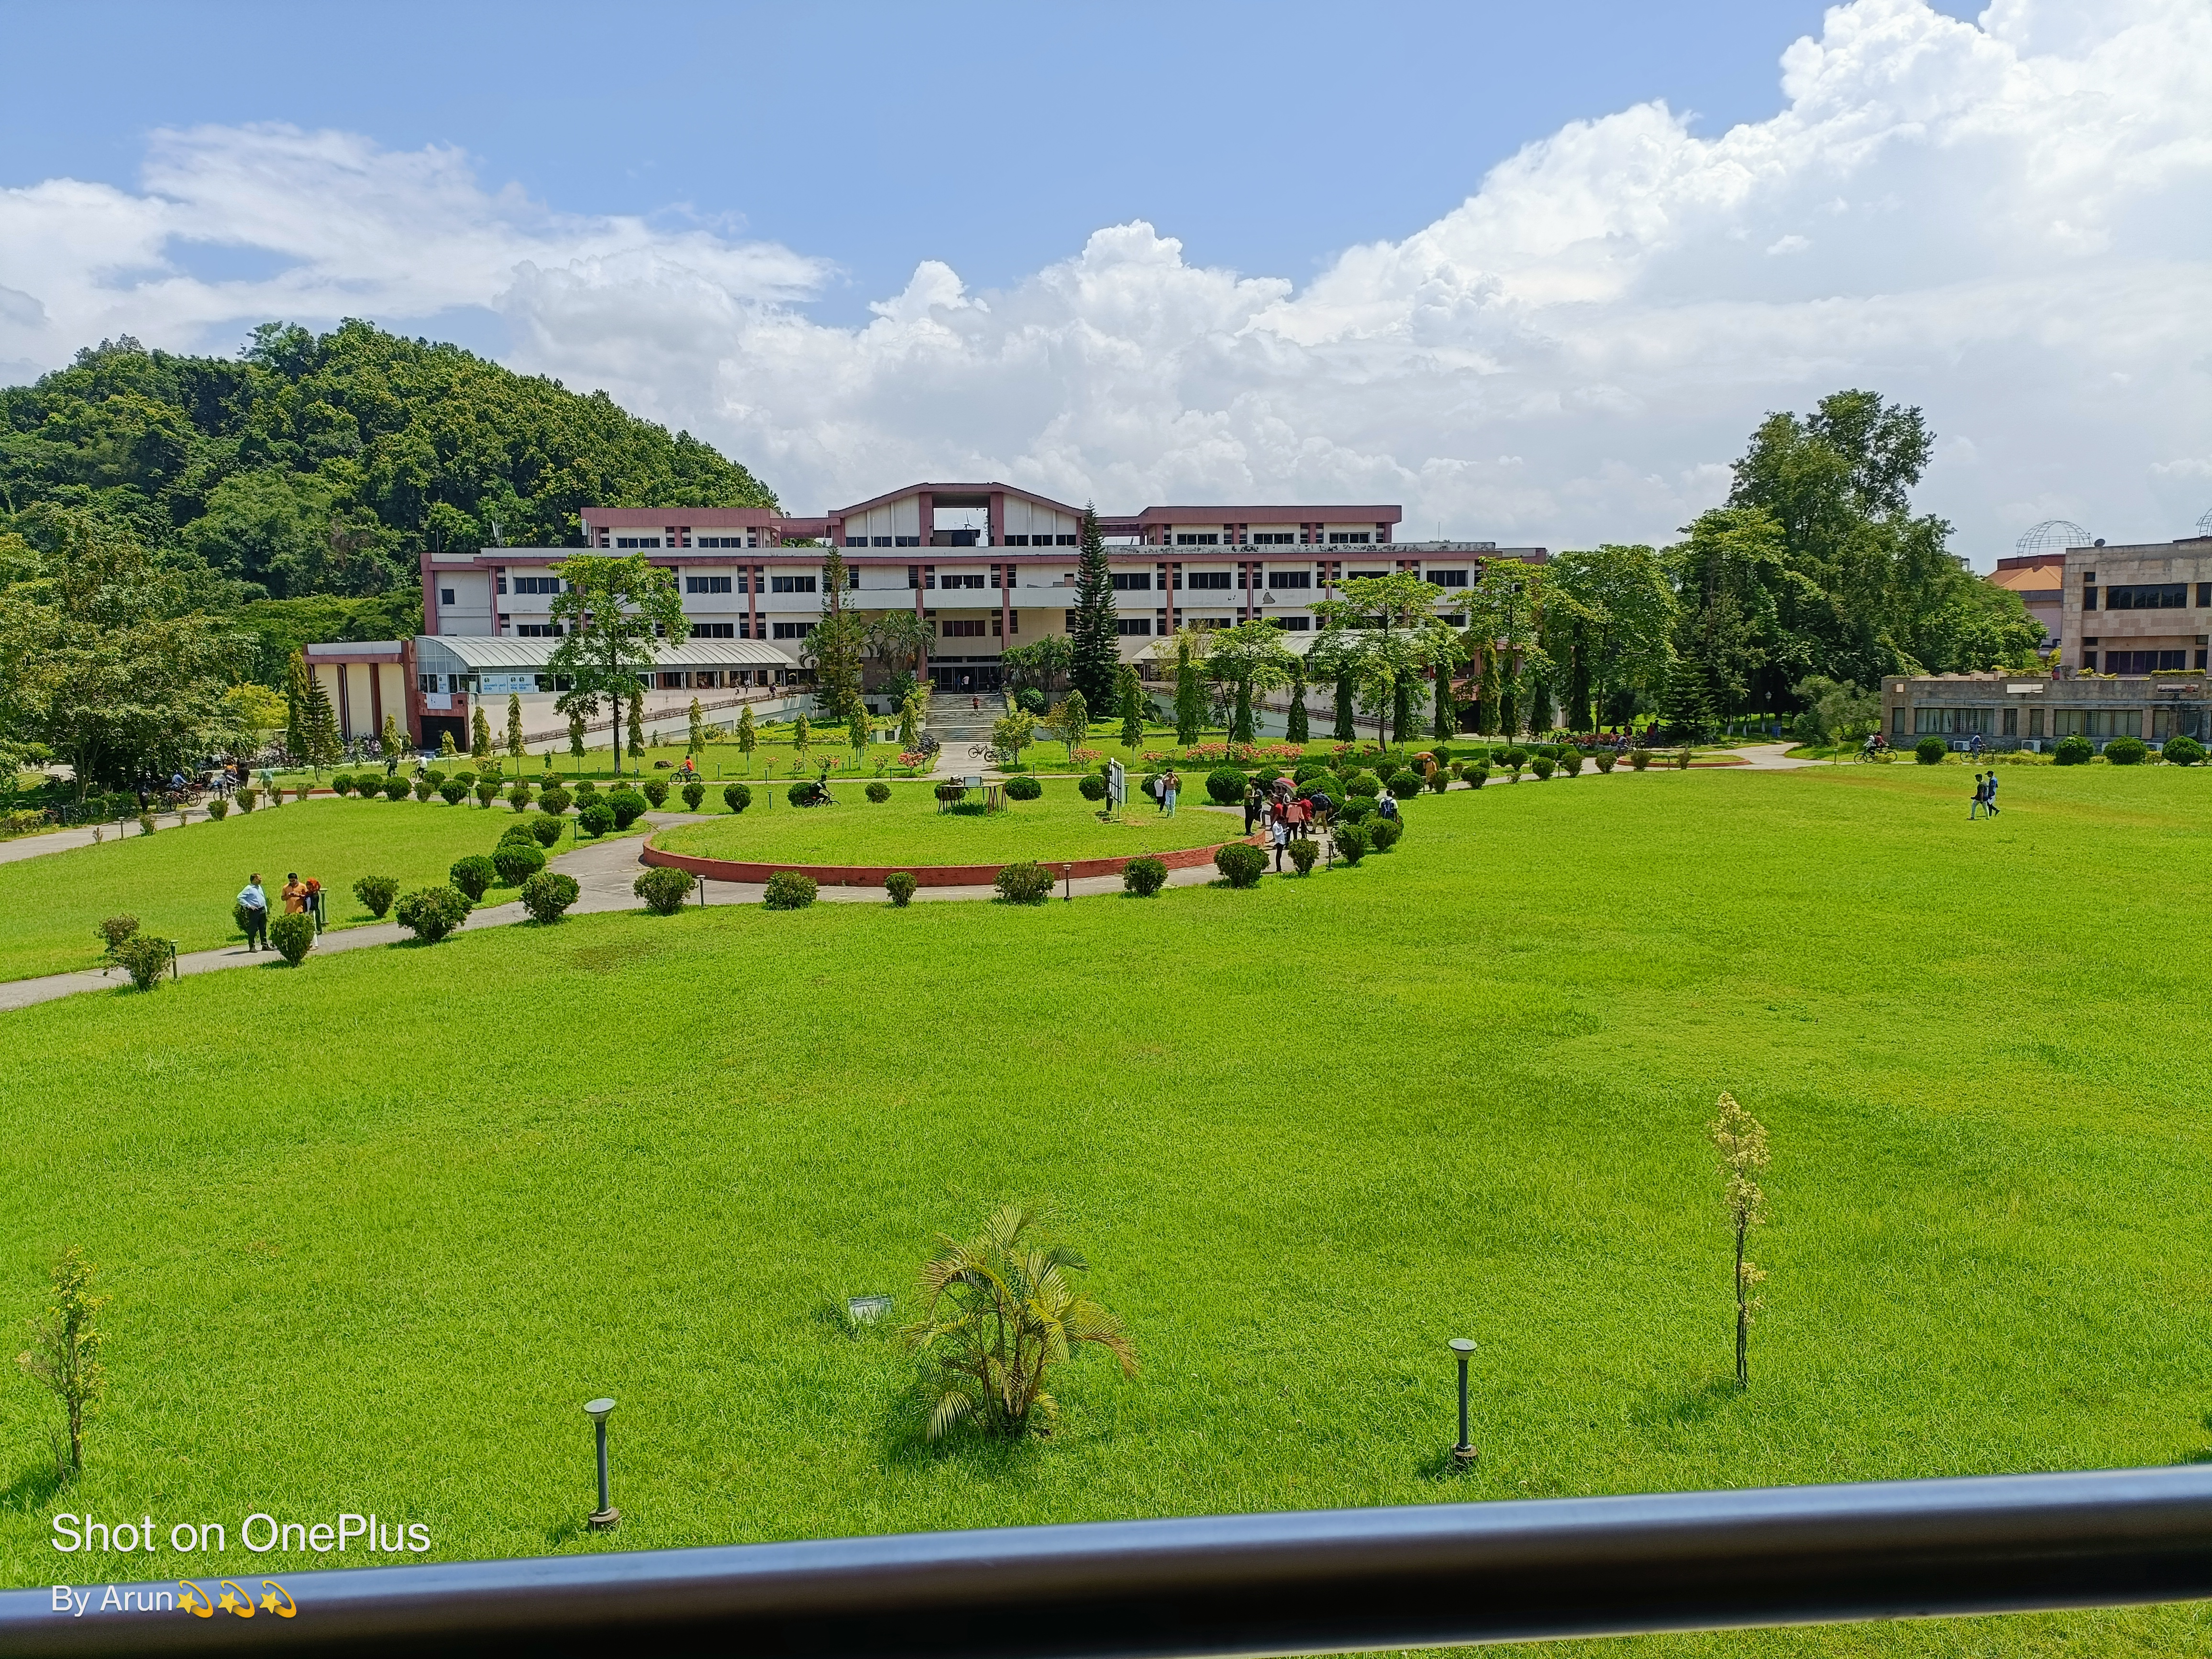
\includegraphics[scale=0.04]{iitg.jpg}
			\caption{IITG LIBRARY}
		\end{subfigure}
		\begin{subfigure}{0.5\textwidth}
			\centering
			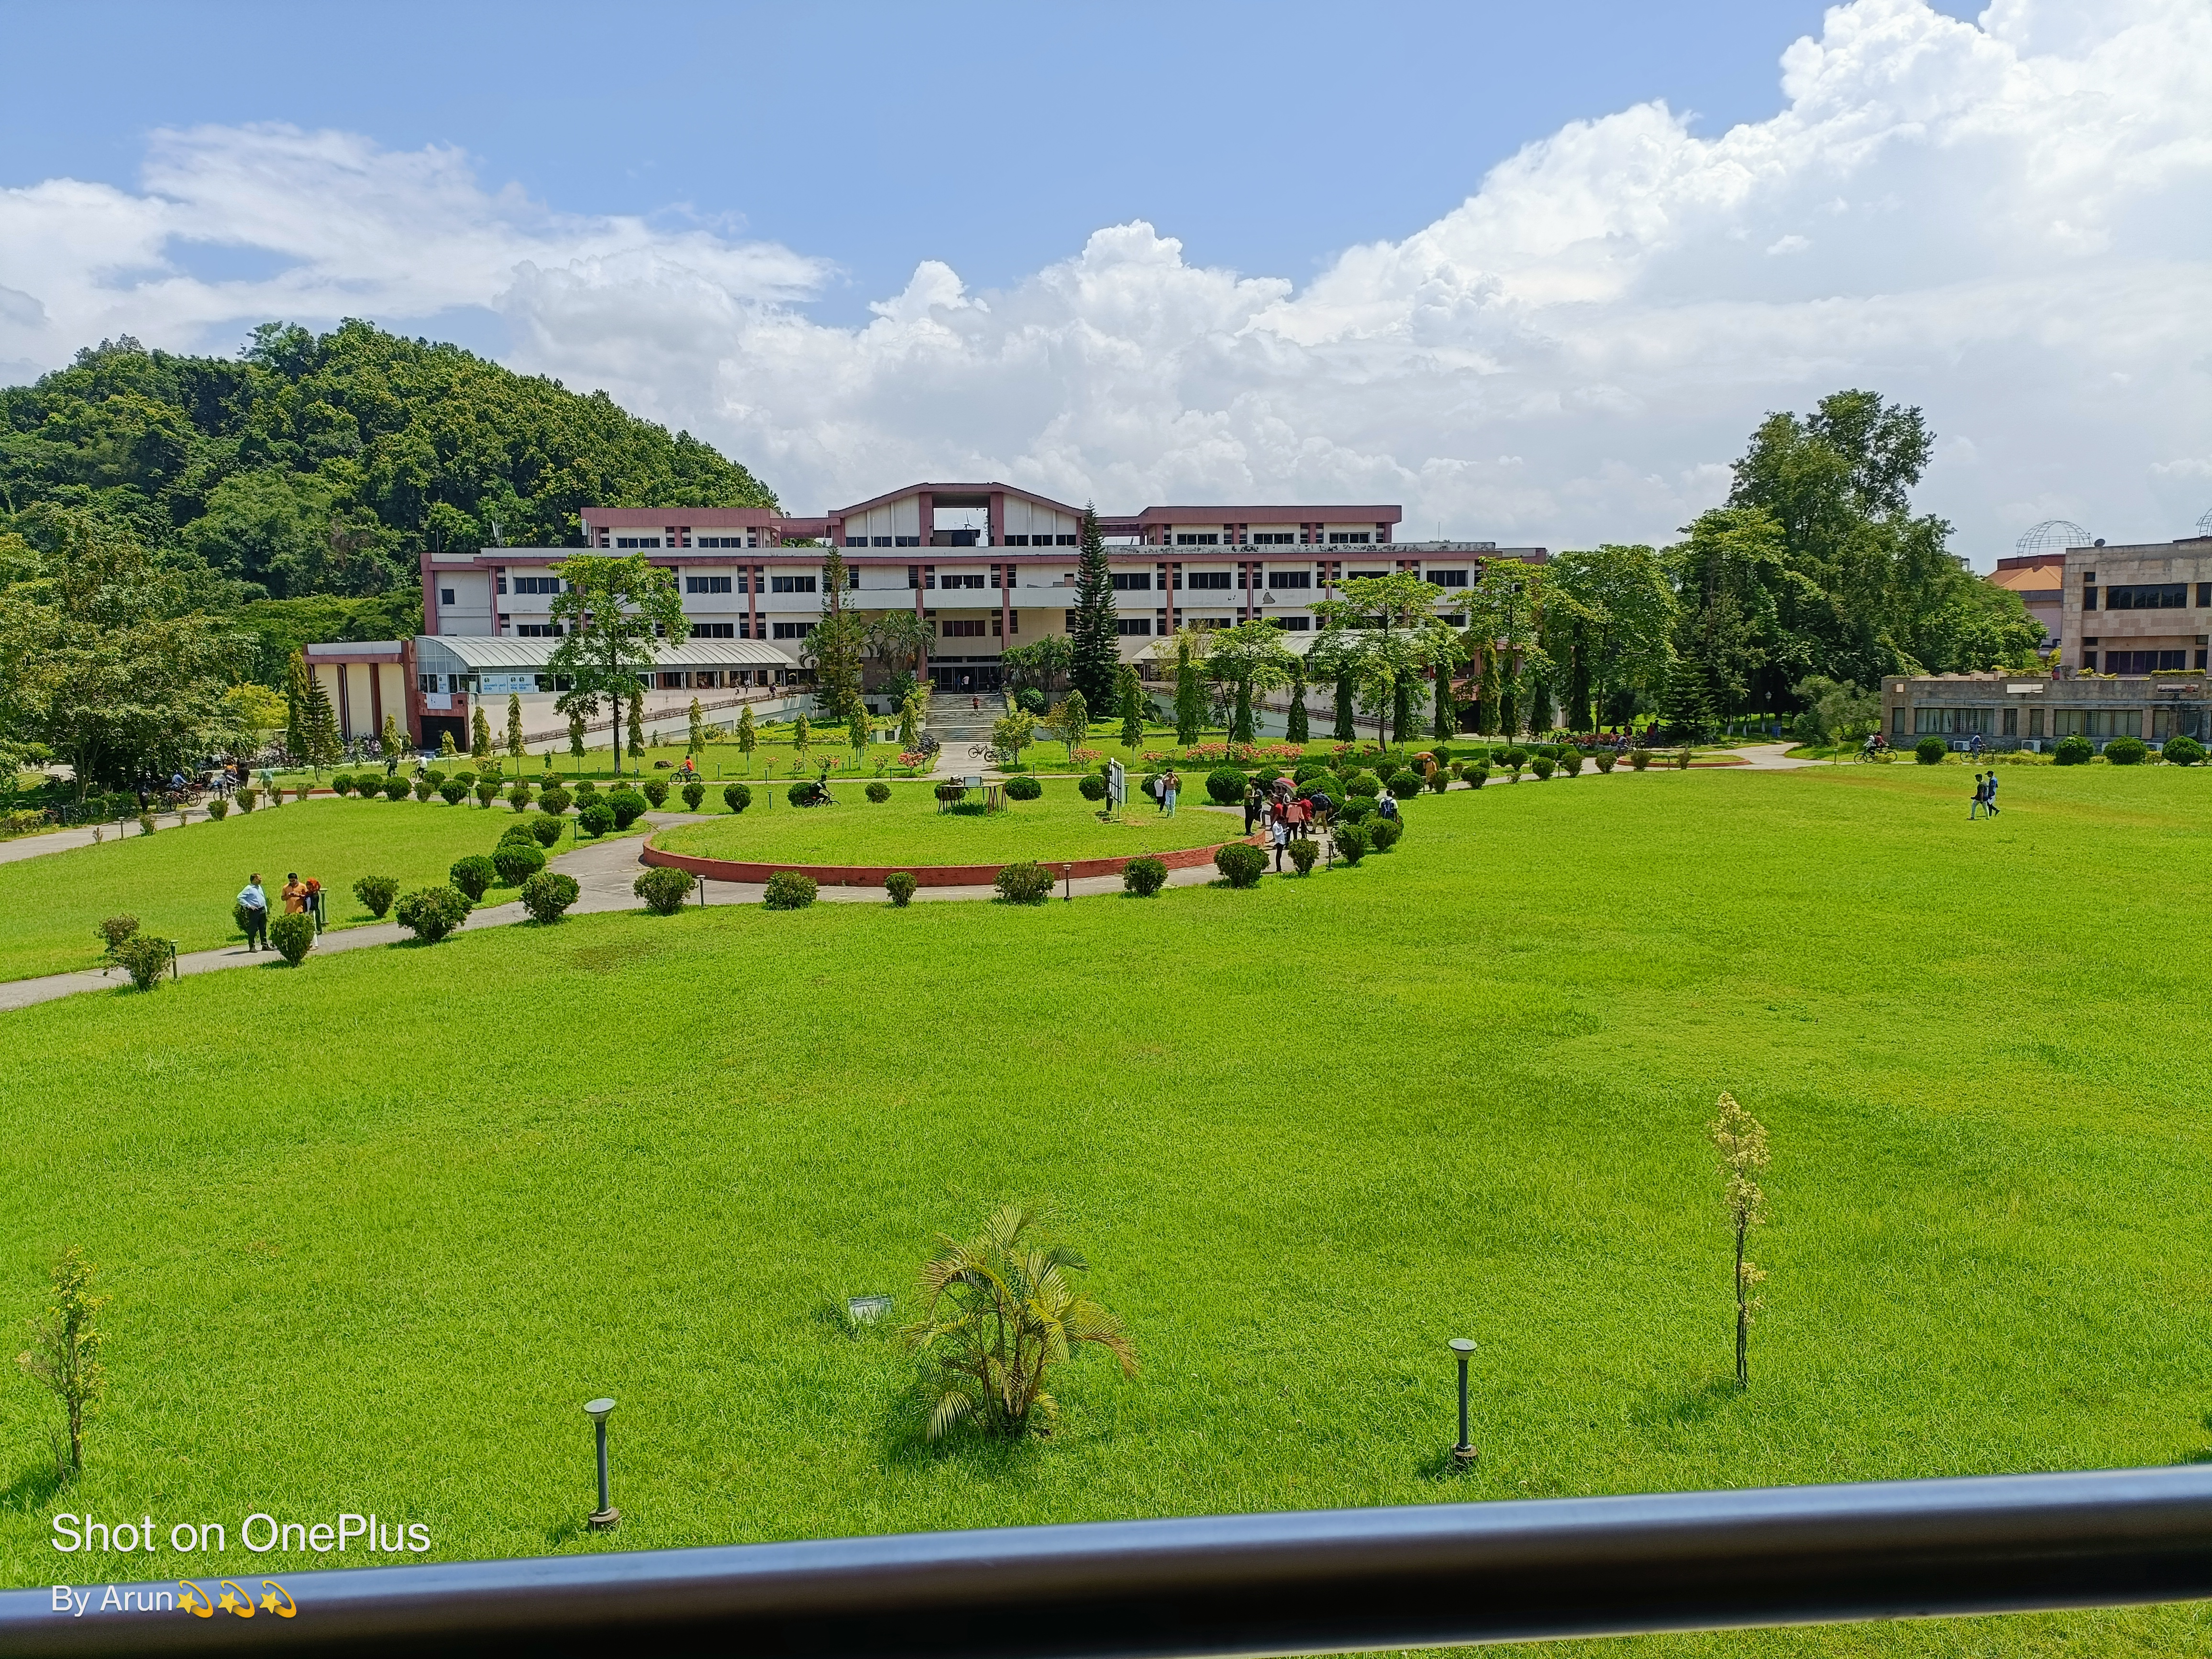
\includegraphics[scale=0.04]{iitg.jpg}
			\caption{IITG LIBRARY}
		\end{subfigure}
		\caption{IITG}
	\end{figure}            
	
	\newpage
	chemical Formula \\
	\newline
	\chemfig{A>:[1]B-[-1]C}
	\chemfig{A>:[:45]B-[:-80]C}
	\\
	Regular Polygon
	
	\chemfig{A*5(-B=C-D-E=)}
	
	\begin{figure}[h]
		\centering
		\chemfig{A*5(-B=C-D-E=)}
		\caption{Chemical Formula}
	\end{figure}    
	%\section{New section}
	
	
	\newpage
	
	\section{Table in Latex}
	
	\begin{tabular}{|c|c|c|}
		\hline
		Name & Age & Height\\ \hline
		A  & 23 & 176 \\ \hline
		B  & 24 & 175 \\ \hline
		C  & 25 & 177\\ \hline
		D  & 36 & 178 \\ \hline
	\end{tabular}
	
	\vspace{3mm}
	Next we will see table with caption
	
	Table With Caption
	\begin{table}[h]
		\centering
		\caption{First Latex Table}
		\begin{tabular}{|c|c|c|}
			\hline
			Name & Age & Height\\ \hline
			A  & 23 & 176 \\ \hline
			B  & 24 & 175 \\ \hline
			C  & 25 & 177\\ \hline
			D  & 36 & 178 \\ \hline
		\end{tabular}
	\end{table}

	\newpage
	\section{\centering Table with booktabs}
	\begin{table}[h]
		\centering\caption{My table}
		\begin{tabular}{c|c|c}
			\toprule[2pt]
			Name & Age & Height\\ 
			\midrule[1.5pt]
			A  & 23 & 176 \\ \midrule
			B  & 24 & 175 \\ \midrule
			C  & 25 & 177\\ \midrule
			D  & 36 & 178 \\ 
			\bottomrule[1.5pt]
		\end{tabular}
	\end{table}     
	
	\newpage
	
	\begin{table}[h]
		\centering\textbf{Table Row stretching}
		\centering\caption{My table}
		{
			\renewcommand{\arraystretch}{2}
			
			\begin{tabular}{c|c|c}
				\toprule[2pt]
				Name & Age & Height\\ 
				\midrule[1.5pt]
				A  & 23 & 176 \\ \midrule
				B  & 24 & 175 \\ \midrule
				C  & 25 & 177\\ \midrule
				D  & 36 & 178 \\ 
				\bottomrule[1.5pt]
			\end{tabular}
		}
	\end{table} 
	
	\begin{comment}
		
	
	\begin{table}[h]
		{
			\centering Do vertical stretch
			\caption{My table}
			\renewcommand{\arraystretch}{2}  
			\begin{tabular}{m{3cm}|m{4cm}|m{2cm}}
				\toprule[2pt]
				Name & Age & Height\\ 
				\midrule[1.5pt]
				A  & 23 & 176 \\ \midrule
				B  & 24 & 175 \\ \midrule
				C  & 25 & 177\\ \midrule
				D  & 36 & 178 \\ 
				\bottomrule[1.5pt]
			\end{tabular}
		}
	\end{table} 
	
	  \newpage
	  \begin{table}[h]
	  	\centering\caption{My table}
	  	\begin{tabular} to 0.8\textwidth {x[c]|x[c]|x[c]}
	  		\toprule[2pt]
	  		Name & Age & Height\\ 
	  		\midrule[1.5pt]
	  		A  & 23 & 176 \\ \midrule
	  		B  & 24 & 175 \\ \midrule
	  		C  & 25 & 177\\ \midrule
	  		D  & 36 & 178 \\ 
	  		\bottomrule[1.5pt]
	  	\end{tabular}
	  \end{table}   
	
	
	
\end{comment}
	\newpage
	
	\section{Algorithm in Latex}
	
	\begin{algorithm}
		\caption{New Algorithm}
		\begin{algorithmic}
			\FOR{i=$1$ to $n$}
			\WHILE{$j \le m$}
			\STATE initialize $w$
			\STATE input $x$
			\ENDWHILE
			\ENDFOR
			\end{algorithmic}
		\end{algorithm}	
	
	\section{Algorithm 2 in latex}
	\textbf{Input} : Observation vector y\\
	\textbf{input} : Channel estimate h
	
	\begin{algorithm}
	\caption{New Algorithm}
	\begin{algorithmic}
		\STATE Input 1: Observation vector y
		\STATE Input 2: Channel estimate h
		\STATE 1:REPEAT
		\STATE 2:   compute
		\STATE 3:   compute
				
	\end{algorithmic}
	\end{algorithm}

\newpage
\section{math mode basic}
Inline mode and Display mode\\
We have to write $a^2 + b^2 = c^2$ math formula.
$a^{24}$\\
we now write $\int_{0}^{x}(1 + x^2)$,
$\prod_{0}^{x}(1 + x)$, $\sum_{0}^{x} (1 + x)$


$$ \prod_{0}^{x}(1 + x)$$\\
$$\sum_{0}^{x} (1 + x)$$\\
$$\int_{0}^{x}(1 + x^2)$$\\
$$\int\limits_{0}^{x}(1 + x^2)$$\\

\begin{equation}
	\sqrt{a^2 + b^2} = c
\end{equation}
\begin{equation}
	\frac{a}{b} = c
\end{equation}

\newpage\begin{equation}
	\frac{a}{b}
	\label{eqn:fraction equation}
\end{equation}

\newpage
\section{Referring equation, table, figure, algorithm}
refer equation~\ref{eqn:fraction equation}.
\end{document}
